%*----------- SLIDE -------------------------------------------------------------
\begin{frame}[t]{A problem} 
    \transdissolve[duration=0.5]
    Subsea pipe monitoring is an important application for the oil and gas industry to carry out \textbf{maintenance} that can \textbf{predict great damage} to the environment and monetary loss.

   
    %\newline
        \begin{columns}[t]
            
            \column{0.5\linewidth}
            \begin{center}
            \begin{figure}
                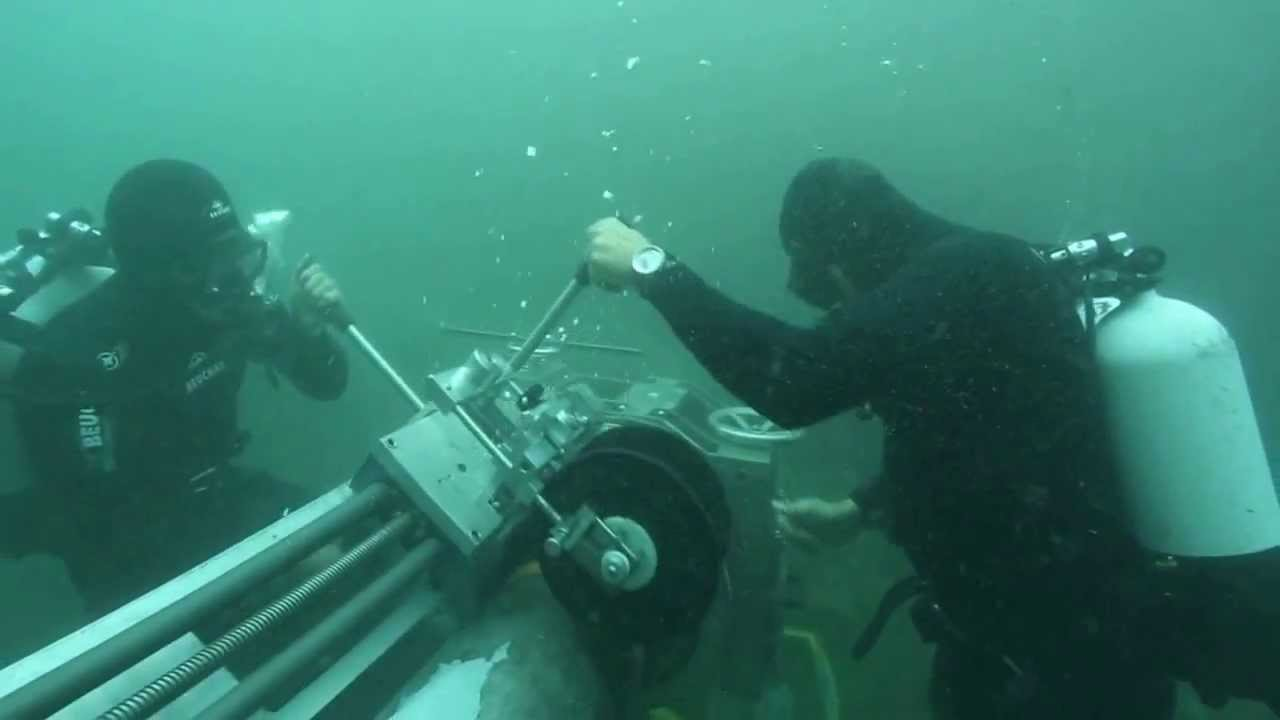
\includegraphics[width=0.8\textwidth]{man_pipeline.jpg}
               
               
                  
               
            \end{figure}

            \end{center}
            \column{.50\linewidth}
            %\vspace*{0.6cm}
            \begin{center}
          
                \begin{figure}
                    
                    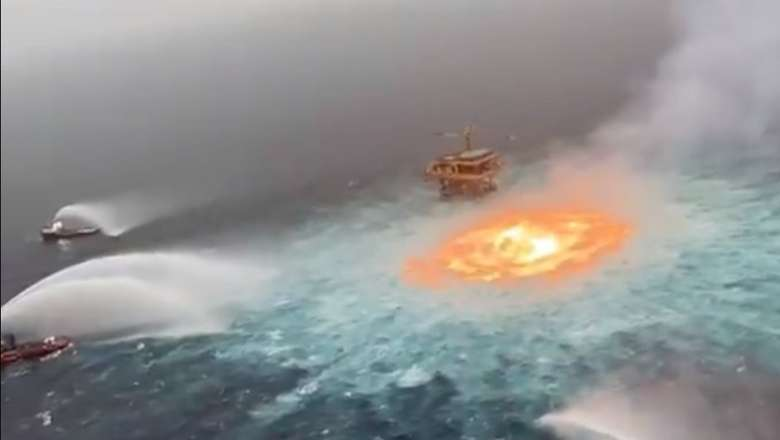
\includegraphics[width=0.8\textwidth]{leak.jpg}
                \end{figure}
            %}
            \end{center}
            
           
        \end{columns}
%*----------- notes
    \note[item]{Notes can help you to remember important information. Turn on the notes option.}
\end{frame}
%-
%*----------- SLIDE -------------------------------------------------------------
\begin{frame}[t]{A solution} 

    Underwater robotics are a good way to try solve this problem or at least minimize.



    \begin{center}
        \begin{figure}
            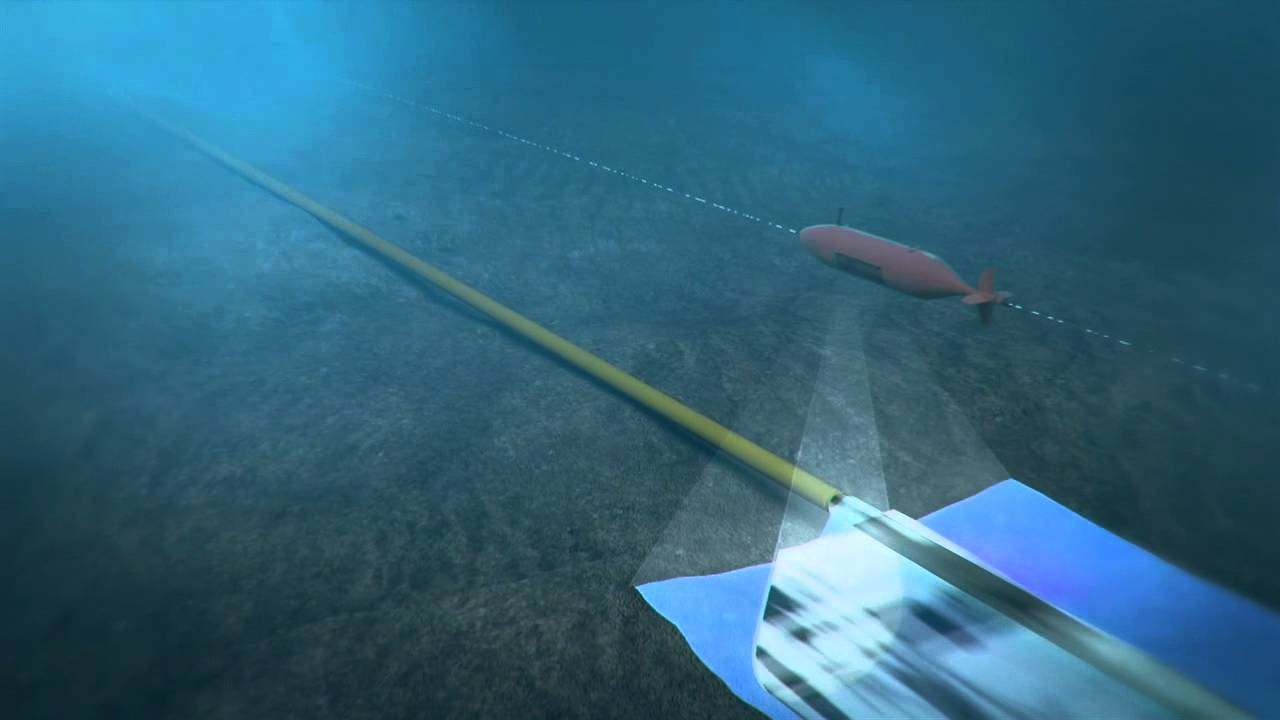
\includegraphics[width=0.65\textwidth]{inspection.jpg}               
           
        \end{figure}

        \end{center}
    
   % \transdissolve[duration=0.5]
   %
   % \begin{center}
   %     \Wider{%
   %     \begin{shaded}
   %     \begin{center}
   %         \vspace*{0.5cm}
   %         \resizebox{!}{0.5cm}{%
   %             \color{bg} The training of researchers in underwater robotics
   %         }%
   %     \end{center}
   %     \end{shaded}
   %     }%
   % \end{center}

\end{frame}


\begin{frame}[t]{The Challenges} 
   The tasks the should be implement is operate a pipefollwing using  undewrater vehicle BlueROv in a simulation at Gazebo.

   There are two challenges: \\
   \begin{itemize}

      \item A global
      \item A focused on undewater robotics field
   \end{itemize}

   \begin{center}
    \begin{figure}
        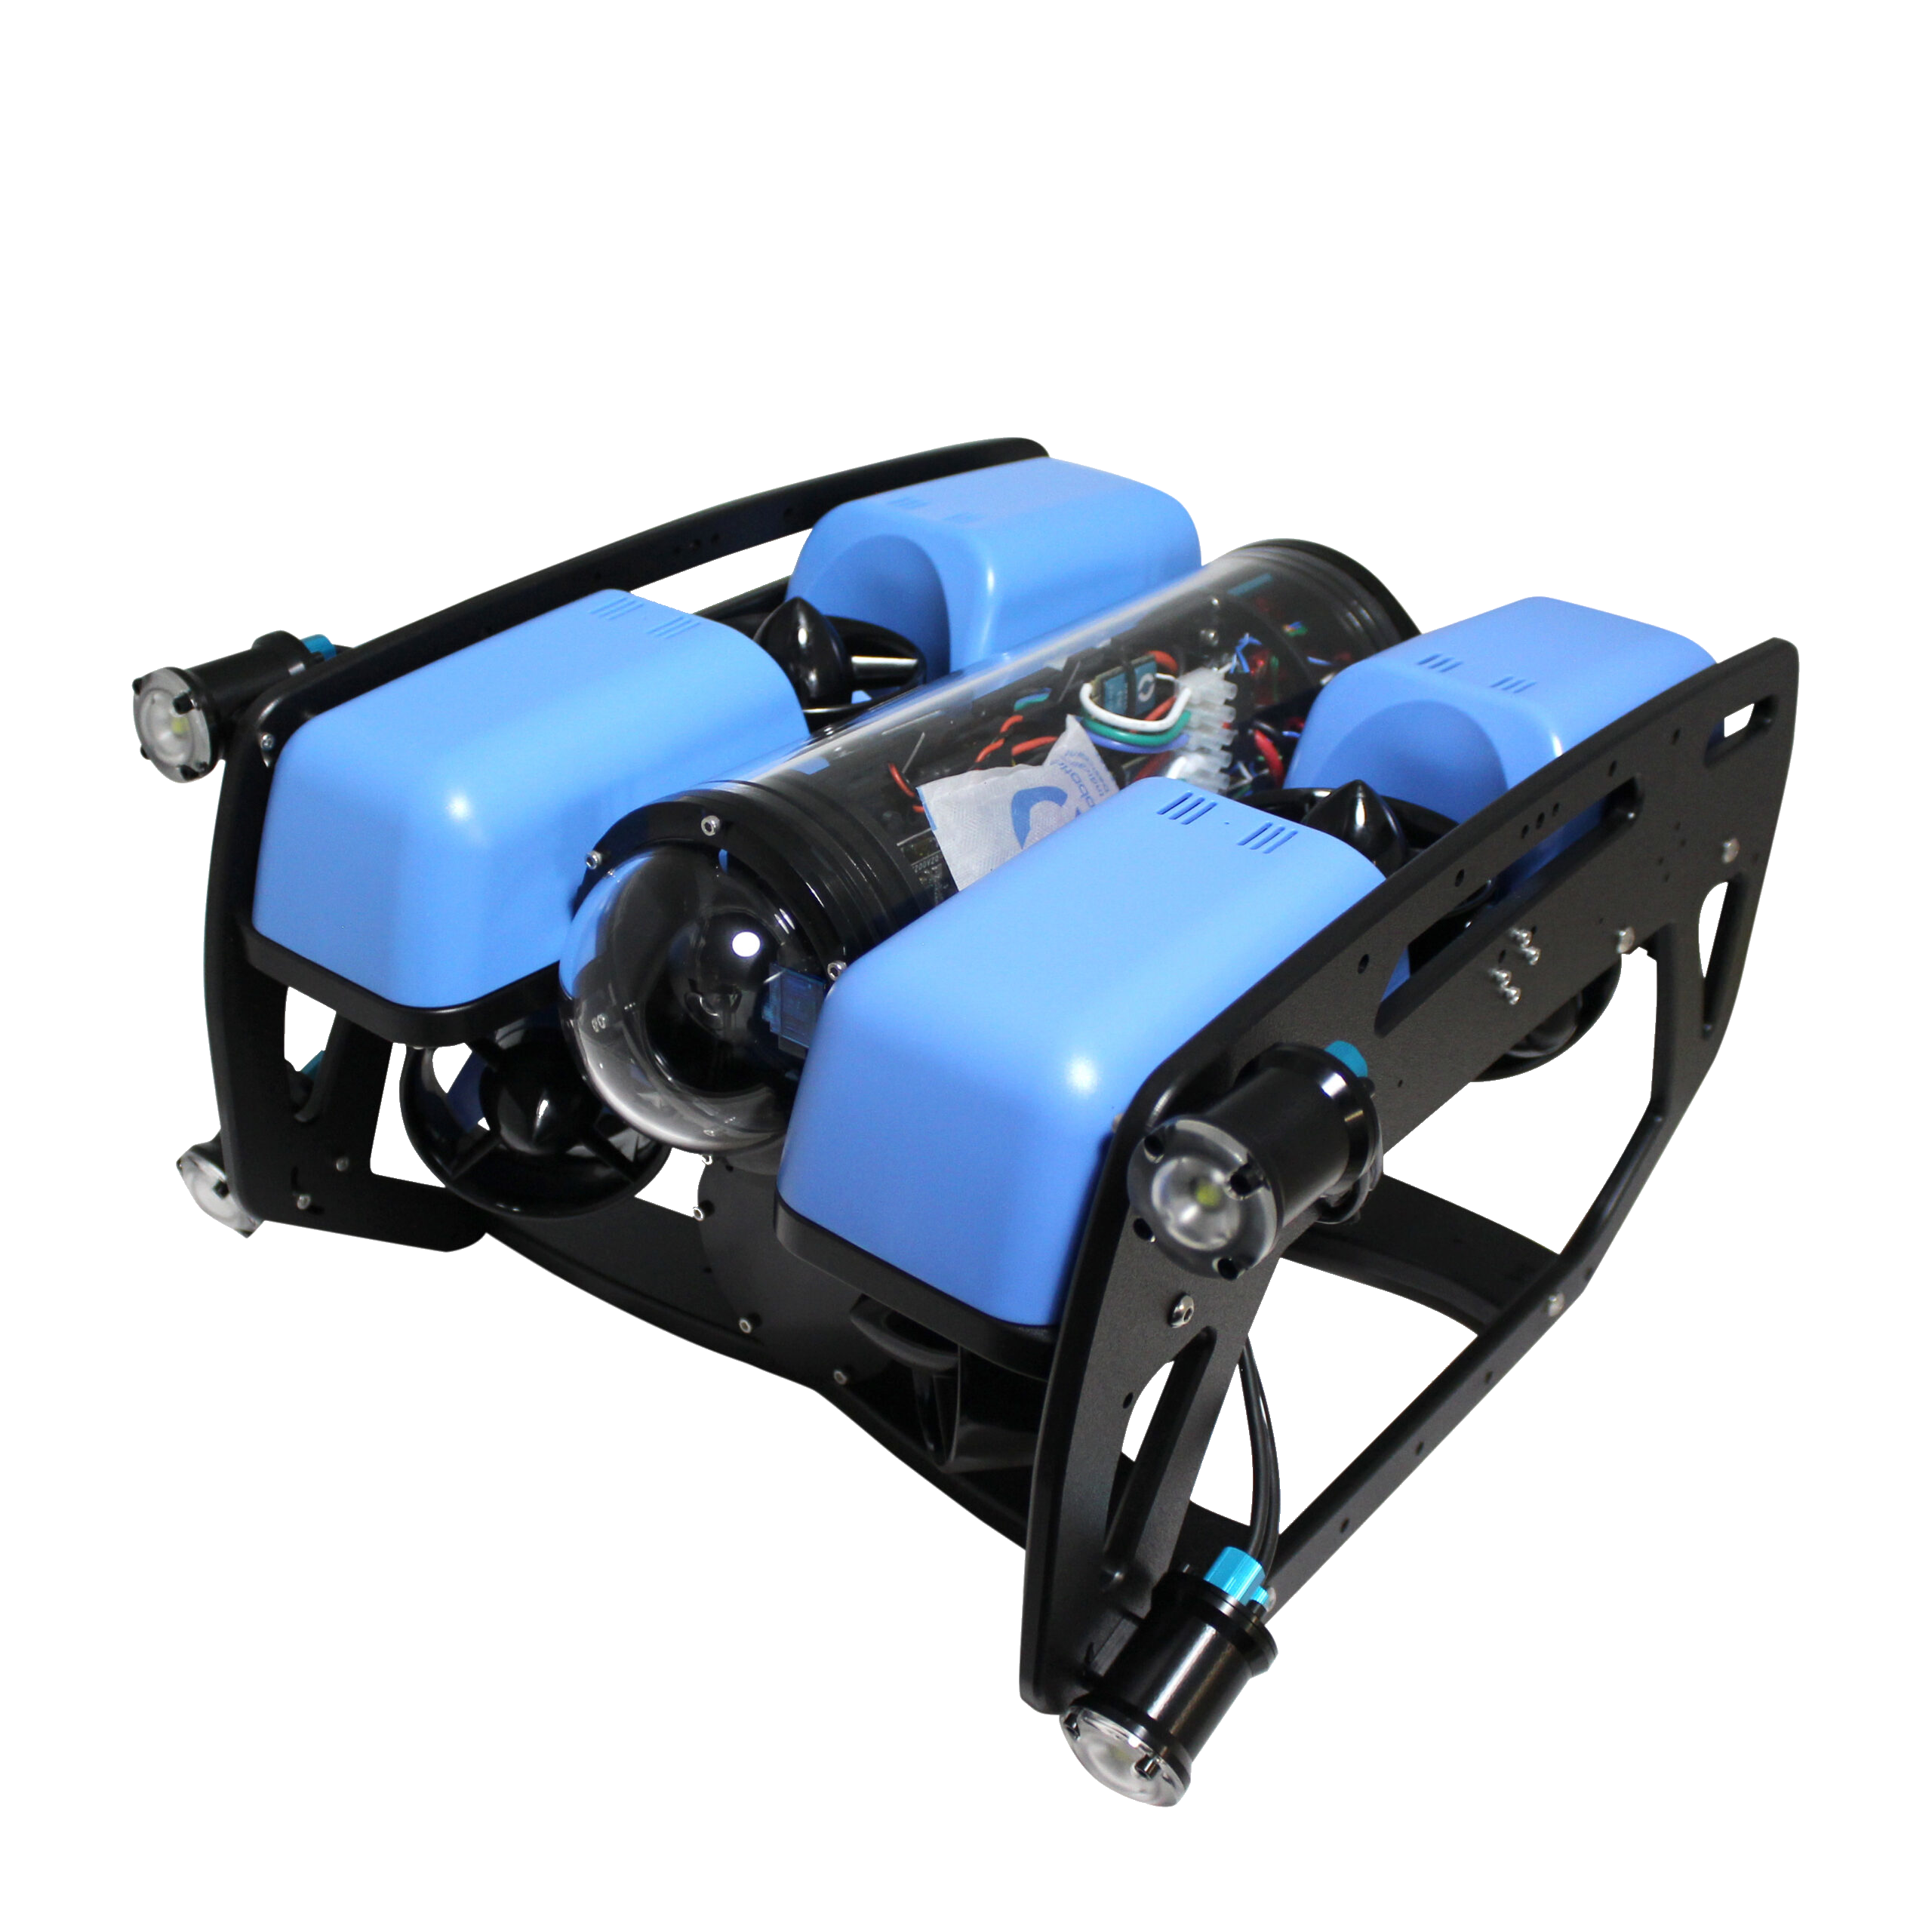
\includegraphics[width=0.8\textwidth]{bluerov.png}               
       
    \end{figure}

    \end{center}


\end{frame}


\begin{frame}{}
    \transdissolve[duration=0.5]
   
    \begin{center}
        \Wider{%
        \begin{shaded}
        \begin{center}
            \vspace*{0.5cm}
            \resizebox{!}{0.5cm}{%
                \color{bg} Global Challenge
            }%
        \end{center}
        \end{shaded}
        }%
    \end{center}
\end{frame}



\begin{frame}{}
    This challenge is broken down into \textbf{two stages}. The first checks the displacement of the vehicle from the initial point of the simulation to the initial pose of the identification of the pipe \textbf{autonomously}. The second is \textbf{monitoring the pipeline}. Artag will be placed at the initial and final point of identification



    \begin{center}
        \begin{figure}
            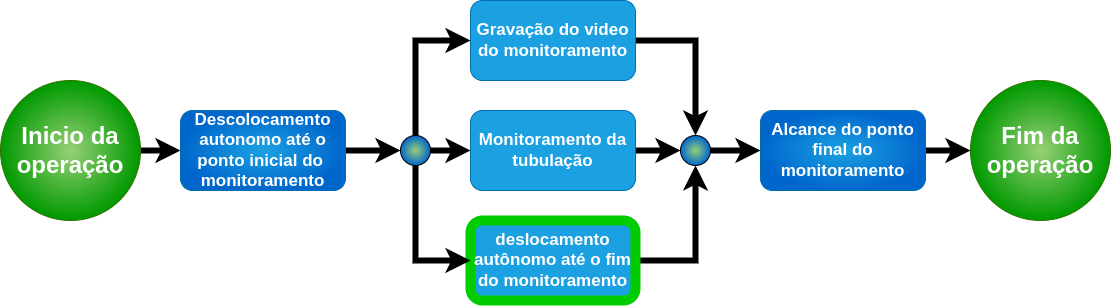
\includegraphics[width=0.8\textwidth]{filed.png}               
           
        \end{figure}
    
        \end{center}
   
\end{frame}

\begin{frame}[t]{Minimal requiriments}
    It is necessary to have:
    \begin{itemize}
        \item a intermiadry knowlogdein ROS 
        \item C++ and/or Python
        \item Computer Vision
        \item Will
    \end{itemize} 
\end{frame}

\begin{frame}{Gains}
   
\end{frame}

\begin{frame}{}
    \transdissolve[duration=0.5]
   
    \begin{center}
        \Wider{%
        \begin{shaded}
        \begin{center}
            \vspace*{0.5cm}
            \resizebox{!}{0.5cm}{%
                \color{bg} Field Challenge
            }%
        \end{center}
        \end{shaded}
        }%
    \end{center}
\end{frame}



\begin{frame}{}

    the Challenge has the objective of carrying out the identification of 100\% of the tentative work, that is, the objective of performing human intervention operations.
   
    \begin{center}
        \begin{figure}
            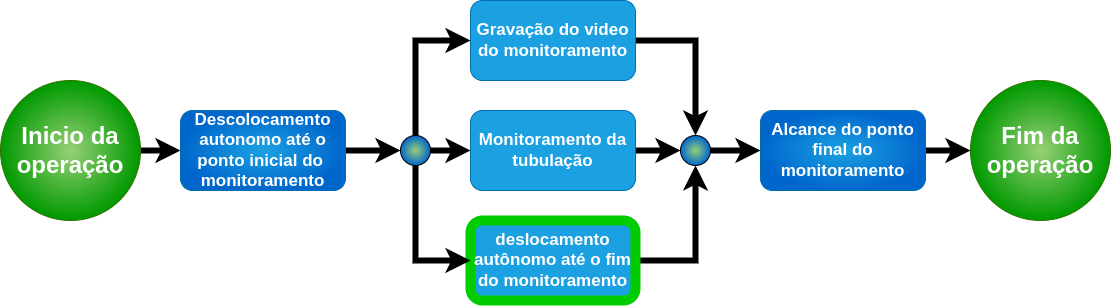
\includegraphics[width=0.8\textwidth]{filed.png}               
           
        \end{figure}
    
        \end{center}
\end{frame}

\begin{frame}{Minimal requiriments}
    It is necessary to have:
    \begin{itemize}
        \item a intermiadry knowlogdein ROS 
        \item C++ and/or Python
        \item Computer Vision
        \item Will
    \end{itemize} 
   
\end{frame}

\begin{frame}{Gains}
    \begin{itemize}
        \item  knowlogde in ROS 
        \item  knowlogde and exprience in robotics.
        \item Computer Vision
        \item underwaterrobotics
        \item Will
    \end{itemize} 
   
\end{frame}






    
   
